\documentclass[11pt]{article}
\usepackage[a4paper,margin=25mm]{geometry}
\usepackage{amsmath,amssymb,mathtools,booktabs,array,xcolor,hyperref,tikz}
\usetikzlibrary{arrows.meta,positioning}
\definecolor{ndblue}{HTML}{174A7E}
\definecolor{ndgreen}{HTML}{2E7D32}
\definecolor{ndgray}{HTML}{F2F4F7}
\hypersetup{colorlinks=true,linkcolor=ndblue,citecolor=ndgreen,urlcolor=ndblue}
\newcommand{\R}{\mathbb R}
\newcommand{\C}{\mathbb C}
\newcommand{\normh}[1]{\left\lVert#1\right\rVert_h}
\newcommand{\lean}[1]{\texttt{\detokenize{#1}}}

\title{A Formalization Milestone:\\A Machine-Checked Convergence Chain for a
Periodic\\Cayley--Crank--Nicolson Discretization}
\author{R.R.\\NDEA Formalization Project}
\date{30 August 2026}

\begin{document}
\maketitle

\begin{abstract}
We report a Lean~4.31 formalization connecting the main components of a
classical convergence analysis for a periodic one-dimensional
Cayley--Crank--Nicolson discretization of the linear Schr\"odinger equation.
This formalization milestone includes the periodic centered finite-difference
Laplacian, Cayley-factor invertibility and unitarity, arbitrary finite-step
weighted-norm stability, explicit spatial and temporal Taylor remainder
estimates, a fixed-time $O(k^2+h^2)$ bound, and grid-family convergence.  The
numerical theorem is classical.  The contribution is the audited Lean~4
formalization.  Any claim that this is the first formalization of its exact
kind remains preliminary and unchecked.  The principal declarations compile
without \texttt{sorry}, \texttt{admit}, custom axioms, or
\texttt{native\_decide}.
\end{abstract}

\section{Scope and contribution}

\begin{center}
\fcolorbox{ndblue}{ndgray}{\parbox{0.88\textwidth}{
\textbf{Status of this document.} This is a formalization milestone.
The numerical theorem is classical.  The contribution is the audited Lean~4
formalization.  Any ``first'' claim remains preliminary and unchecked.}}
\end{center}

A paper proof of numerical PDE convergence crosses analytic Taylor estimates,
finite periodic indexing, complex matrix algebra, stability, and asymptotic
reasoning.  Machine checking forces the interfaces between these layers to be
explicit.  This development connects six verified stages:
\begin{enumerate}
  \item the periodic centered finite-difference Laplacian;
  \item Cayley-factor invertibility and unitarity;
  \item arbitrary finite-step weighted-norm stability;
  \item explicit spatial and temporal Taylor remainder estimates;
  \item a fixed-time $O(k^2+h^2)$ error estimate; and
  \item a grid-family convergence result.
\end{enumerate}
The work does not claim a new numerical method or analytic convergence order.
Formal convergence of other finite-difference PDE schemes has been achieved in
Coq~\cite{Boldo2013,Tekriwal2021}.  The present contribution is the particular
audited end-to-end Lean chain and its reusable interfaces.  Public searches
have not established priority, and no definitive ``first'' claim is made.

\section{Continuous problem and discrete update}

Let $U:\R\times\R\to\C$ satisfy
\begin{equation}\label{eq:pde}
  \partial_tU(t,x)=i\,\partial_{xx}U(t,x),\qquad
  U(t,x+L)=U(t,x),\qquad L>0.
\end{equation}
For $m+1$ periodic nodes, let $h=L/(m+1)$ and let
$H_h=-\Delta_h$ be the centered periodic negative Laplacian.  For $k>0$, put
\[
 A=I+i\frac{k}{2}H_h,\qquad B=I-i\frac{k}{2}H_h,\qquad Q=BA^{-1}.
\]
The numerical trajectory satisfies $v^{j+1}=Qv^j$, and
\[
 \normh{w}=\left(h\sum_i|w_i|^2\right)^{1/2}.
\]

\section{The machine-checked chain}

\begin{figure}[ht]
\centering
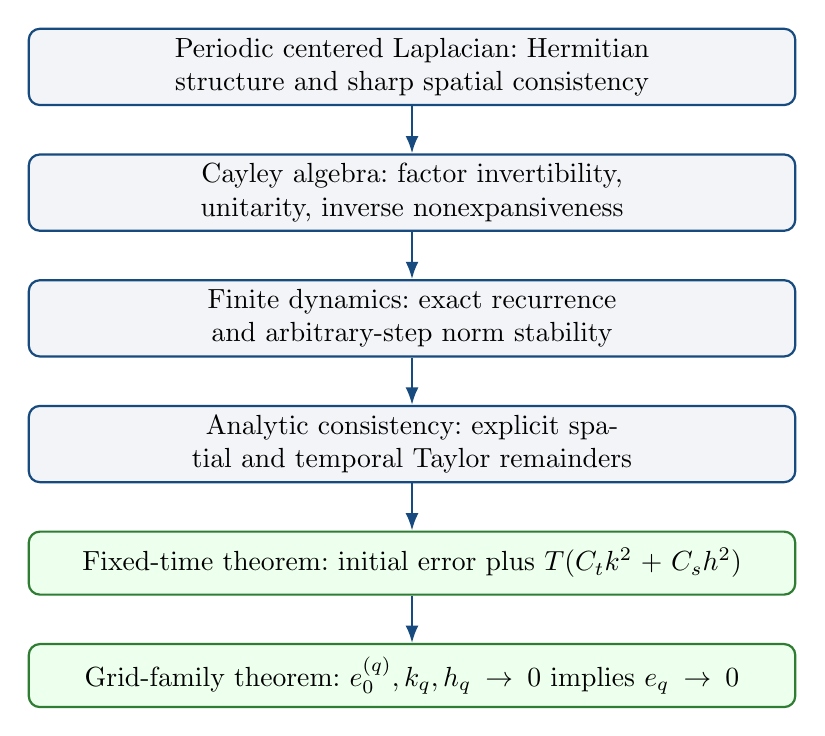
\begin{tikzpicture}[
 node distance=6mm,
 box/.style={draw=ndblue,thick,rounded corners,fill=ndgray,
   align=center,text width=95mm,minimum height=8mm},
 last/.style={box,draw=ndgreen,fill=green!7},
 arr/.style={-{Latex[length=2.2mm]},thick,draw=ndblue}]
\node[box] (lap) {Periodic centered Laplacian:\ Hermitian structure and sharp spatial consistency};
\node[box,below=of lap] (cay) {Cayley algebra:\ factor invertibility, unitarity, inverse nonexpansiveness};
\node[box,below=of cay] (stab) {Finite dynamics:\ exact recurrence and arbitrary-step norm stability};
\node[box,below=of stab] (tay) {Analytic consistency:\ explicit spatial and temporal Taylor remainders};
\node[last,below=of tay] (fixed) {Fixed-time theorem:\ initial error plus $T(C_tk^2+C_sh^2)$};
\node[last,below=of fixed] (grid) {Grid-family theorem:\ $e_0^{(q)},k_q,h_q\to0$ implies $e_q\to0$};
\draw[arr] (lap)--(cay); \draw[arr] (cay)--(stab);
\draw[arr] (stab)--(tay); \draw[arr] (tay)--(fixed);
\draw[arr] (fixed)--(grid);
\end{tikzpicture}
\caption{The verified dependency spine.}
\label{fig:chain}
\end{figure}

\subsection{Periodic centered Laplacian}

For a periodic grid vector $w$,
\[
 (H_hw)_i=\frac{2w_i-w_{i+1}-w_{i-1}}{h^2},
\]
with indices interpreted cyclically.  The development proves the index
identities, invariance of finite sums under shifts, the matrix action formula,
Hermiticity and positive semidefiniteness of $H_h$, and summation by parts.

\subsection{Cayley invertibility, unitarity, and finite stability}

Hermiticity gives the Gram identity needed to prove that $A$ is invertible.
The formal proof constructs $A^{-1}$ internally and verifies both multiplication
identities.  It then proves
\[
 Q^*Q=I,\qquad QQ^*=I.
\]
Thus $Q$ preserves both Euclidean and weighted norms, while $A^{-1}$ is
nonexpansive in the norm used for residual accumulation.  For an explicitly
recursive $N$-step update, induction proves
\begin{equation}\label{eq:stability}
 \normh{Q^Nw}=\normh{w}.
\end{equation}
The dimension and the number of steps are quantified rather than computed at a
single finite instance.

\subsection{Explicit Taylor estimates}

Assume the uniform derivative bounds
\[
 |\partial_x^4U(t,x)|\le M_s,\qquad
 |\partial_t^3U(t,x)|\le M_t.
\]
The two spatial integral remainders satisfy
\[
 |R_+(x,h)|\le\frac{M_sh^4}{24},\qquad
 |R_-(x,h)|\le\frac{M_sh^4}{24}.
\]
Cancellation of the odd terms and division by $h^2$ gives
\begin{equation}\label{eq:space}
 \left|(-\Delta_hu)(x)+u''(x)\right|
 \le\frac{M_s}{12}h^2.
\end{equation}
Periodic sampling and $(m+1)h=L$ yield
\begin{equation}\label{eq:spaceweighted}
 \normh{r_s^j}\le\sqrt L\,\frac{M_s}{12}h^2.
\end{equation}
For the normalized Crank--Nicolson temporal defect, the verified Taylor
assembly yields
\begin{equation}\label{eq:time}
 \normh{r_t^j}\le\sqrt L\,\frac{5M_t}{12}k^2.
\end{equation}
The analytic-closure module derives the needed interval statements from global
$C^3$ time regularity rather than assuming remainder estimates externally.

\section{Fixed-time error estimate}

Let $u_h^j$ sample $U(jk,\cdot)$ and set $e^j=u_h^j-v^j$.  The PDE identity,
averaged spatial profile, and consistency estimates give the exact residual
\[
 Au_h^{j+1}=Bu_h^j+kr^j.
\]
Applying $A^{-1}$ gives
\[
 e^{j+1}=Qe^j+A^{-1}(kr^j),\qquad
 \normh{e^{j+1}}\le\normh{e^j}+k\normh{r^j}.
\]
Iteration and $Nk\le T$ prove
\begin{equation}\label{eq:main}
\boxed{
 \normh{e^N}\le\normh{e^0}
 +T\left[
   \sqrt L\,\frac{5M_t}{12}k^2
   +\sqrt L\,\frac{M_s}{12}h^2
 \right].}
\end{equation}
The Lean declaration is
\lean{periodic_cayley_cn_convergence_of_smooth_solution}.

\section{Grid-family convergence}

For a family indexed by $q$, if
\[
 e_0^{(q)}\to0,\qquad k_q\to0,\qquad h_q\to0,
\]
then the explicit right-hand side of~\eqref{eq:main} tends to zero.  A squeeze
argument gives convergence of the numerical error.  Exact initialization is a
specialized corollary.

\section{Lean artifact and assurance}

\begin{center}
\begin{tabular}{>{\raggedright\arraybackslash}p{0.40\textwidth}
                >{\raggedright\arraybackslash}p{0.50\textwidth}}
\toprule
Module & Role \\
\midrule
\small\texttt{PeriodicCayleyCN-}\newline\texttt{AnalyticClosureV1} &
  Smooth PDE solution to fixed-time estimate \\
\small\texttt{PeriodicCayleyCN-}\newline\texttt{ConstantModeExampleV1} &
  Exact zero-error constant-mode check \\
\small\texttt{PeriodicCayleyCN-}\newline\texttt{GridFamilyConvergenceV1} &
  Vanishing-mesh convergence consequences \\
\bottomrule
\end{tabular}
\end{center}

The production sources were built with Lean~4.31.0.  Clean-runtime replay,
direct source checks, theorem-signature inspection, and axiom audits were
preserved.  The headline declarations depend only on \texttt{propext},
\texttt{Classical.choice}, and \texttt{Quot.sound}.  The relevant new sources
contain no \texttt{sorry}, \texttt{admit}, custom \texttt{axiom}, or
\texttt{native\_decide}.

Kernel acceptance alone does not ensure that the encoded statement is the
intended one~\cite{Meek2026}.  Accordingly, the project preserves the informal
theorem, explicit constants, dependency map, anti-placeholder checks, and a
prior-art/reviewer packet.  Any priority assessment remains preliminary and
unchecked.

\section{Limitations and conclusion}

The theorem concerns a smooth solution of the linear one-dimensional periodic
equation.  It is not a nonlinear well-posedness theorem, a long-time dispersive
analysis, a floating-point program certificate, or an infinite-dimensional
operator-convergence theorem.

This formalization milestone is a connected, machine-checked account of how
periodic finite
differences, Cayley algebra, stability, Taylor consistency, finite-time
accumulation, and asymptotic convergence fit together.  It provides an
auditable certificate for the stated result and a foundation for further
formal numerical-PDE developments in Lean.

\begin{thebibliography}{9}
\bibitem{Akrivis1993}
G.~D. Akrivis, \emph{Finite difference discretization of the cubic
Schr\"odinger equation}, IMA J. Numer. Anal. 13 (1993), 115--124.
\url{https://doi.org/10.1093/imanum/13.1.115}

\bibitem{Boldo2013}
S.~Boldo, F.~Cl\'ement, J.-C.~Filli\^atre, M.~Mayero, G.~Melquiond, and P.~Weis,
\emph{Wave equation numerical resolution: a comprehensive mechanized proof of
a C program}, J. Automated Reasoning 50 (2013), 423--456.
\url{https://arxiv.org/abs/1001.4898}

\bibitem{Tekriwal2021}
M.~Tekriwal, K.~Duraisamy, and J.-B.~Jeannin,
\emph{A formal proof of the Lax equivalence theorem for finite difference
schemes}, 2021. \url{https://arxiv.org/abs/2103.13534}

\bibitem{Meek2026}
T.~Meek, S.~Ge, D.~Q.~Xiang, S.~Chess, and V.~Ilin,
\emph{Formalizing Numerical Analysis: An Agent Pipeline and Quality Audit
Beyond Kernel Acceptance}, 2026. \url{https://arxiv.org/abs/2606.14000}
\end{thebibliography}

\end{document}
